\documentclass[
    margin=1in,
    innermargin=-4.5in,
    ]{tikzposter}

% Choose size here
\geometry{paperwidth=33.11in,paperheight=46.81in} %A0
% \geometry{paperheight=33.11in,paperwidth=23.4in} %A1
    
\usepackage[utf8]{inputenc}
\usepackage{csquotes}
\usepackage{amsmath}
\usepackage{amsfonts}
\usepackage{amsthm}
\usepackage{amssymb}
\usepackage{mathrsfs}
\usepackage{graphicx}
\usepackage{lipsum}
\usepackage[export]{adjustbox}
\usepackage{tcolorbox}
\usepackage[font=small,labelfont=bf]{caption} % Required for specifying captions to tables and figures
\usepackage{enumitem}
\usepackage[backend=biber,style=numeric]{biblatex}
\usepackage{glasgow-poster-theme}
\makeatletter
\setlength{\TP@visibletextwidth}{31.0in}
\setlength{ \TP@visibletextheight}{45in}
\makeatother
\usepackage{bm}
\usepackage{bbm}

\addbibresource{refs.bib}

% set theme parameters
\tikzposterlatexaffectionproofoff
\usetheme{UniGlasgowTheme}
\usecolorstyle{UniGlasgowStyle}

\usepackage[scaled]{helvet}
\renewcommand\familydefault{\sfdefault} 
\renewcommand{\vec}[1]{\bm{#1}}
\newcommand{\Tr}{\text{Tr}}
\renewcommand{\AA}{\mathcal{A}}
\newcommand{\BB}{\mathcal{B}}
\newcommand{\ZZ}{\mathbb{Z}}
\newcommand{\CC}{\mathbb{C}}
\usepackage[T1]{fontenc}


\title{\parbox{0.8\linewidth}{\Huge \textbf{SPT indices emerging from translation invariance in two dimensional quantum spin systems}}}
\author{Tijl Jappens\textsuperscript{1}}
\institute{\textsuperscript{1}Instituut voor theoretische fysica, Katholieke Universiteit Leuven}

% Adjust trim if title doesn't have two lines
\titlegraphic{
\includegraphics[width=0.35\linewidth, clip]{figures/KU_Leuven_logo.png}}


% begin document
\begin{document}
\maketitle
\centering
\begin{columns}
    \column{0.5}
    \block{Setup}{
       \textbf{An operator algebra} is constructed using:\\
	\begin{tabular}{ l l }
	$\bullet$ A lattice $\Lambda$ ($\ZZ$ or $\ZZ^2$).&$\bullet$An on site Hilbert space $\CC^d$.\\
	$\bullet$For each $\Gamma\subset \Lambda$ finite, a finite algebra$\quad$&$\bullet$The local algebra \\
	$\qquad\AA_\Gamma=\bigotimes_{i\in\Gamma}\BB(\CC^d)$.&$\qquad \AA_{\text{loc}}=\bigcup_{\substack{\Gamma\subset\Lambda\\\text{finite}}}\AA_{\Gamma}$.
	\end{tabular}\\
	The operator algebra is the norm closure of the local algebra $\AA_{\Lambda}=\overline{\AA_{\text{loc}}}$.\\
	\textbf{A group action} is constructed using:\\
	\begin{tabular}{ l l }
	$\bullet$ A group $G$.$\qquad$&$\bullet$A representation of the group: $U\in\textrm{Hom}(G,U(\CC^d))$.
	\end{tabular}\\
	$\bullet$ For each $\Gamma\subset\Lambda$ finite, a finite group action: $\beta_\Gamma(g)=\textrm{Ad}(\bigotimes_{i\in\Gamma}U(g))$\\
	The group action $\beta\in\textrm{Hom}(G,\textrm{Aut}(\AA))$ is defined as $\lim_{\Gamma\rightarrow \Lambda}\beta_\Gamma$.
    }
    
    \block{Method}{
        \begin{center}
            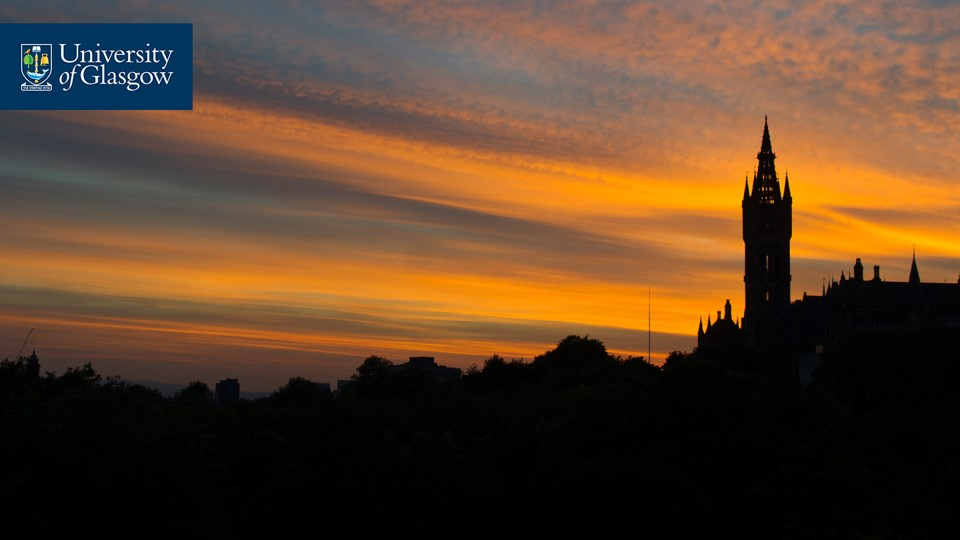
\includegraphics[width=0.8\linewidth]{figures/glasgow_sunset.jpg}
            \captionof{figure}{Sunset in Glasgow}
        \end{center}
        
        \vspace{1cm}
    
        \lipsum[100]
        \lipsum[100]
        \lipsum[100]
    }


    \column{0.5}
    \block{Evaluation}{
        \lipsum[100]
        \lipsum[100]
        \lipsum[100]
        \lipsum[100]
    }

    \block{Conclusions}{
        \lipsum[100]
        \cite{hudak2007history}
        \lipsum[100]
        \lipsum[100]
    }
    
    \block{References}{
            \begin{center}
                   \mbox{}\vspace{-1\baselineskip}
    			\printbibliography[heading=none] 
        	\end{center}
        }

\end{columns}
\end{document}